\documentclass[conference]{IEEEtran}
\usepackage{cite}
\usepackage{url}
\usepackage[cmex10]{amsmath}
\usepackage{algorithm}
\usepackage{algpseudocode}
\usepackage{array}
\usepackage{mdwmath}
\usepackage{mdwtab}
\usepackage{eqparbox}
\usepackage{graphicx,subfigure}
\usepackage {epsfig}
\usepackage{fixltx2e}

\begin{document}

\title{JavaScript Profiling and Optimization on V8}

\author{
\IEEEauthorblockN{Yilin Zhang}
\IEEEauthorblockA{zylime@gmail.com}
\and
\IEEEauthorblockN{C. Vic Hu}
\IEEEauthorblockA{vic@cvhu.org}
}

\maketitle

\begin{abstract}
In this project, we want to focus on the trace profiling and possible optimization to the existing JIT JavaScript engines, such as IonMonkey and V8. By applying the optimization techniques we have learned in class, we want to study how modern browsers dynamically compile JavaScript, and to see if we can come up with a feasible idea to make some enhancements.

\end{abstract}

\section{Introduction}
As the popularity of web-based applications and services increases, browser performance has become one of the major competitions in the industry. Since JavaScript is what makes modern web pages dynamic and interactive, how to optimize its compilation/interpretation is the key component to building fast and robust modern browsers. Apart from its essential role in client-side interactions, JavaScript also became one of the mainstream server-side solutions in recent years\cite{node}. 

Although JavaScript is traditionally translated into byte code by an interpreter, more and more JavaScript Engines in modern browsers  are designed to compile directly into machine code. Our project will mainly focus on trace profiling\cite{Trace} in IonMonkey and V8, and make constructive adjustments according to the optimization techniques we have learned in class. We will use the SunSpider JavaScript Benchmark to measure and compare the existing infrastructure with our proposed optimizations, and make a sound analysis of the results. If time permitting, we will also look into JavaScript Engine solutions on mobile devices. Our overall goal is to understand the common optimization procedures performed by modern JavaScript Engines, as well as the possible performance enhancements with the knowledge we've acquired from EE382V. 

%
%As we know internet riches people's life with new and quick information. At the same time people spend more and more timing browsing various websites. How to make the webpages response faster and save people's time becomes important. Infrastructure of cables and servers definitely play an important role, but compilation optimization\cite{Trace} and arrange the HTML tree\cite{Popularity} make difference when the infrastructure is unchangable.
%
%In this work, we will tackle both compilation optimization and arrangement of the HTML tree to accelerate the web response. We use TraceMonkey to help build the trace information and several optimization techniques are applied based on the trace structure. We analyze the web site popularity from the HTTP log file and then revise the HTTP tree based on the popularity.

%
%\section{Motivation}

JavaScript is slow mainly due to JavaScript programs are untyped, and then compiled and run on the fly. Dynamic compilation is a great complement to static one. But completely replacing the optimized-to-death static compilation with JIT will lose the performance. 
%
%

%%%%%%Prime Algorithm starts here%%%%%%%%%%%%%%%%%%%%%%%%%%%%%%%%%%%%%%%%%%%%%%%%%%%%%%%%%%%%%%%%%%%%

\begin{algorithm}[hbt!]
	\caption{\scriptsize{\emph{Calculate the 25000th Prime Number}}}
	 \label{algorithm:prime}
	 \begin{algorithmic}[1]
%		 \begin{scriptsize}			 
%\If {$i\geq maxval$}
%    \State $i\gets 0$
%\Else
%    \If {$i+k\leq maxval$}
%        \State $i\gets i+k$
%    \EndIf
%\EndIf
			\Require
			 \Ensure {The 25000th Prime Number P}
			 \State {Prime list PL = \{\}} 
			 \For {P = 1 to infinity}
			    \State {Flag = true}
			    \For{index = 1 to PL.size()}
			 	\If {P.mod(PL[i]) == 0}
			            \State {Flag = false}
			            \State {Continue}
			        \EndIf
			    \EndFor
			    \If {Flag == true}
			        \State {PL.push\_back(P)}
			        \If {PL.size() == 25000}
			            \Return {PL.back()}
			        \EndIf
			     \EndIf
			  \EndFor
%		\end{scriptsize}
	\end{algorithmic}
\end{algorithm}

%%%%%%%%%%%%%%%%%%%%%%%%%%%%%%%%%%%%%%%%%%%%%%%%%%%%%%%%%%%%%%%%%%%%%%%%%%%%%%%%%%%%%%%%%%%%%%%%%%
\section{Approach}
JavaScript is slower compared with other programming languages, such as C++. Before applying the optimization to the compilation of JavaScript code, we use one example to analyze how slow JavaScript is compared with the same code in C++. The example we use here is to calculate the 25000th prime number\cite{google_IO}. The overall algorithm of of calculating the 25000th prime number is illustrated in Algorithm\ref{algorithm:prime}.
The corresponding C++ code is in the Fig.\ref{figure:prime_cplusplus} while the JavaScript version is in the Fig.\ref{figure:JavaScript}.

\begin{figure}[hbt!]
	\label{figure:prime}
    \centering
        \subfigure[]{
            \label{figure:prime_cplusplus}
            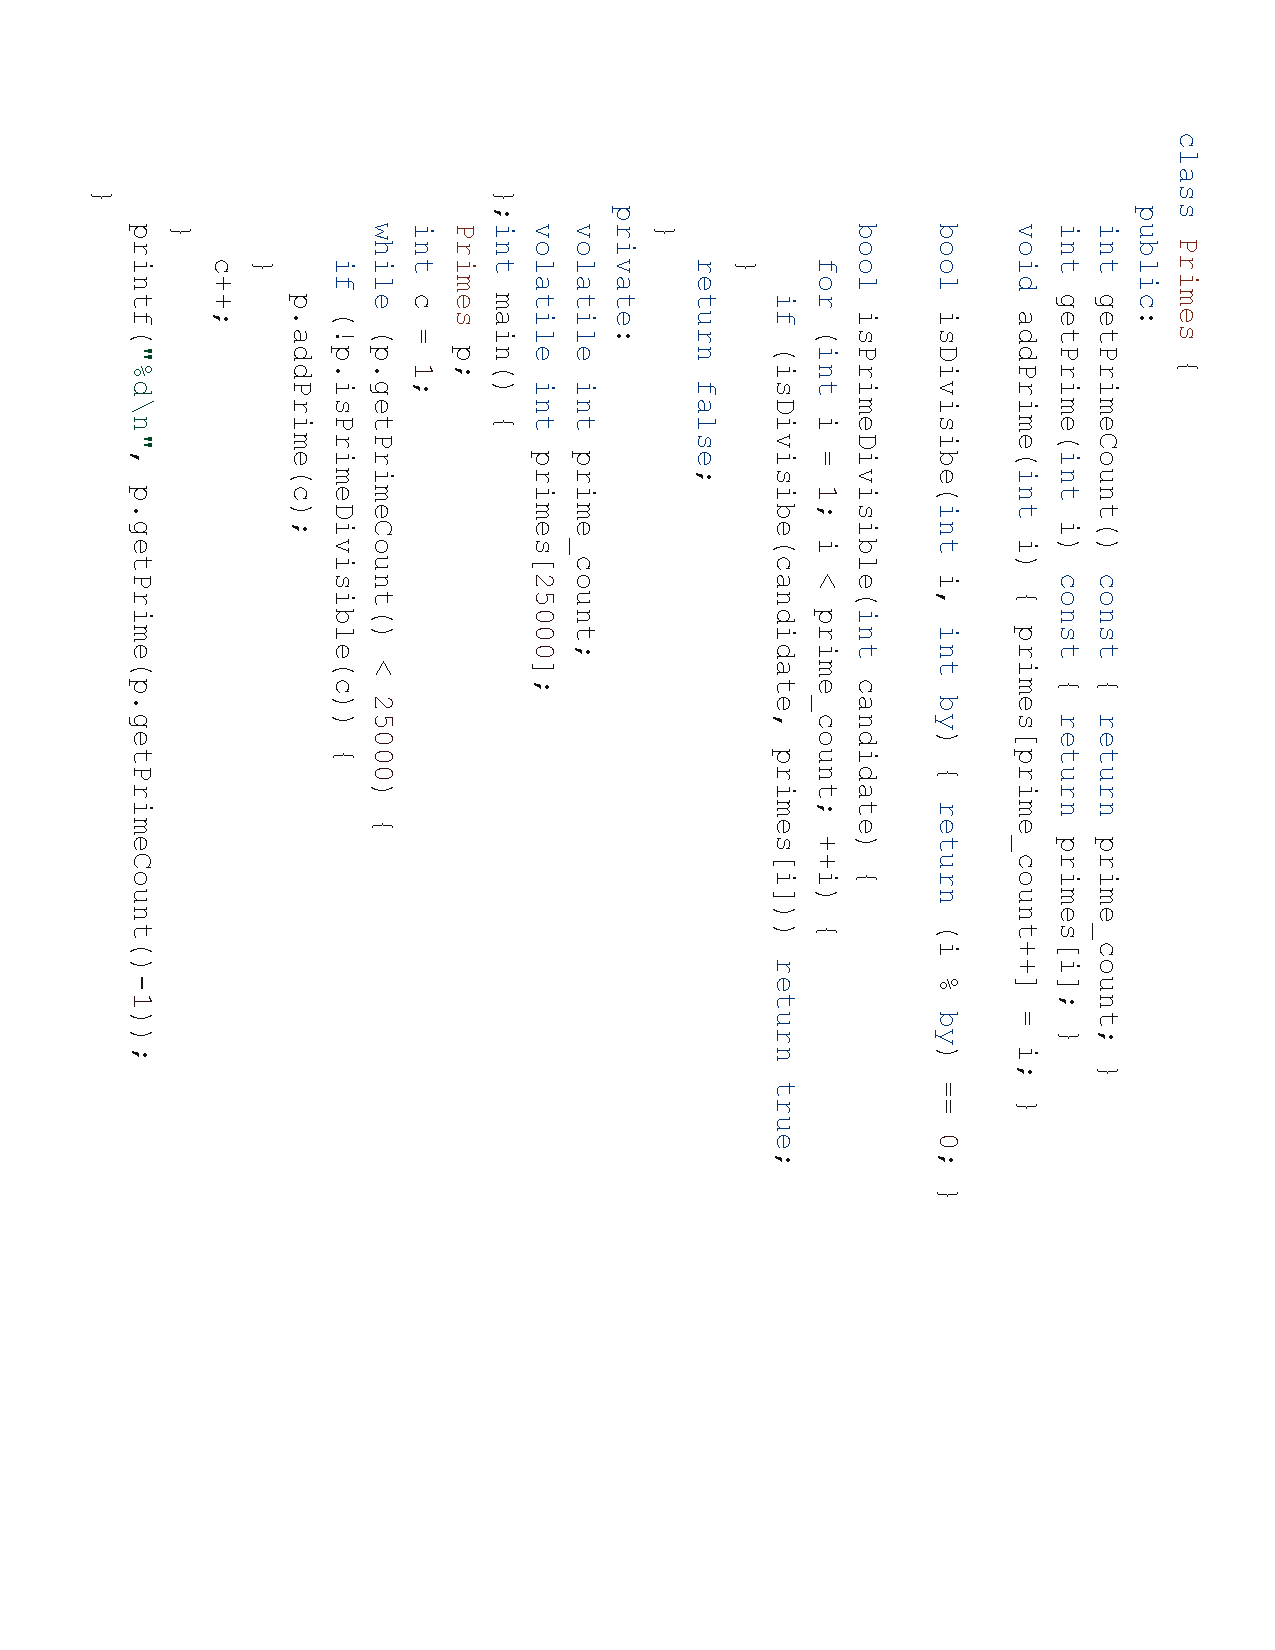
\includegraphics[width=0.44\textwidth]{figs/prime_cplusplus}
        }
        \subfigure[]{
           \label{figure:prime_JavaScript}
           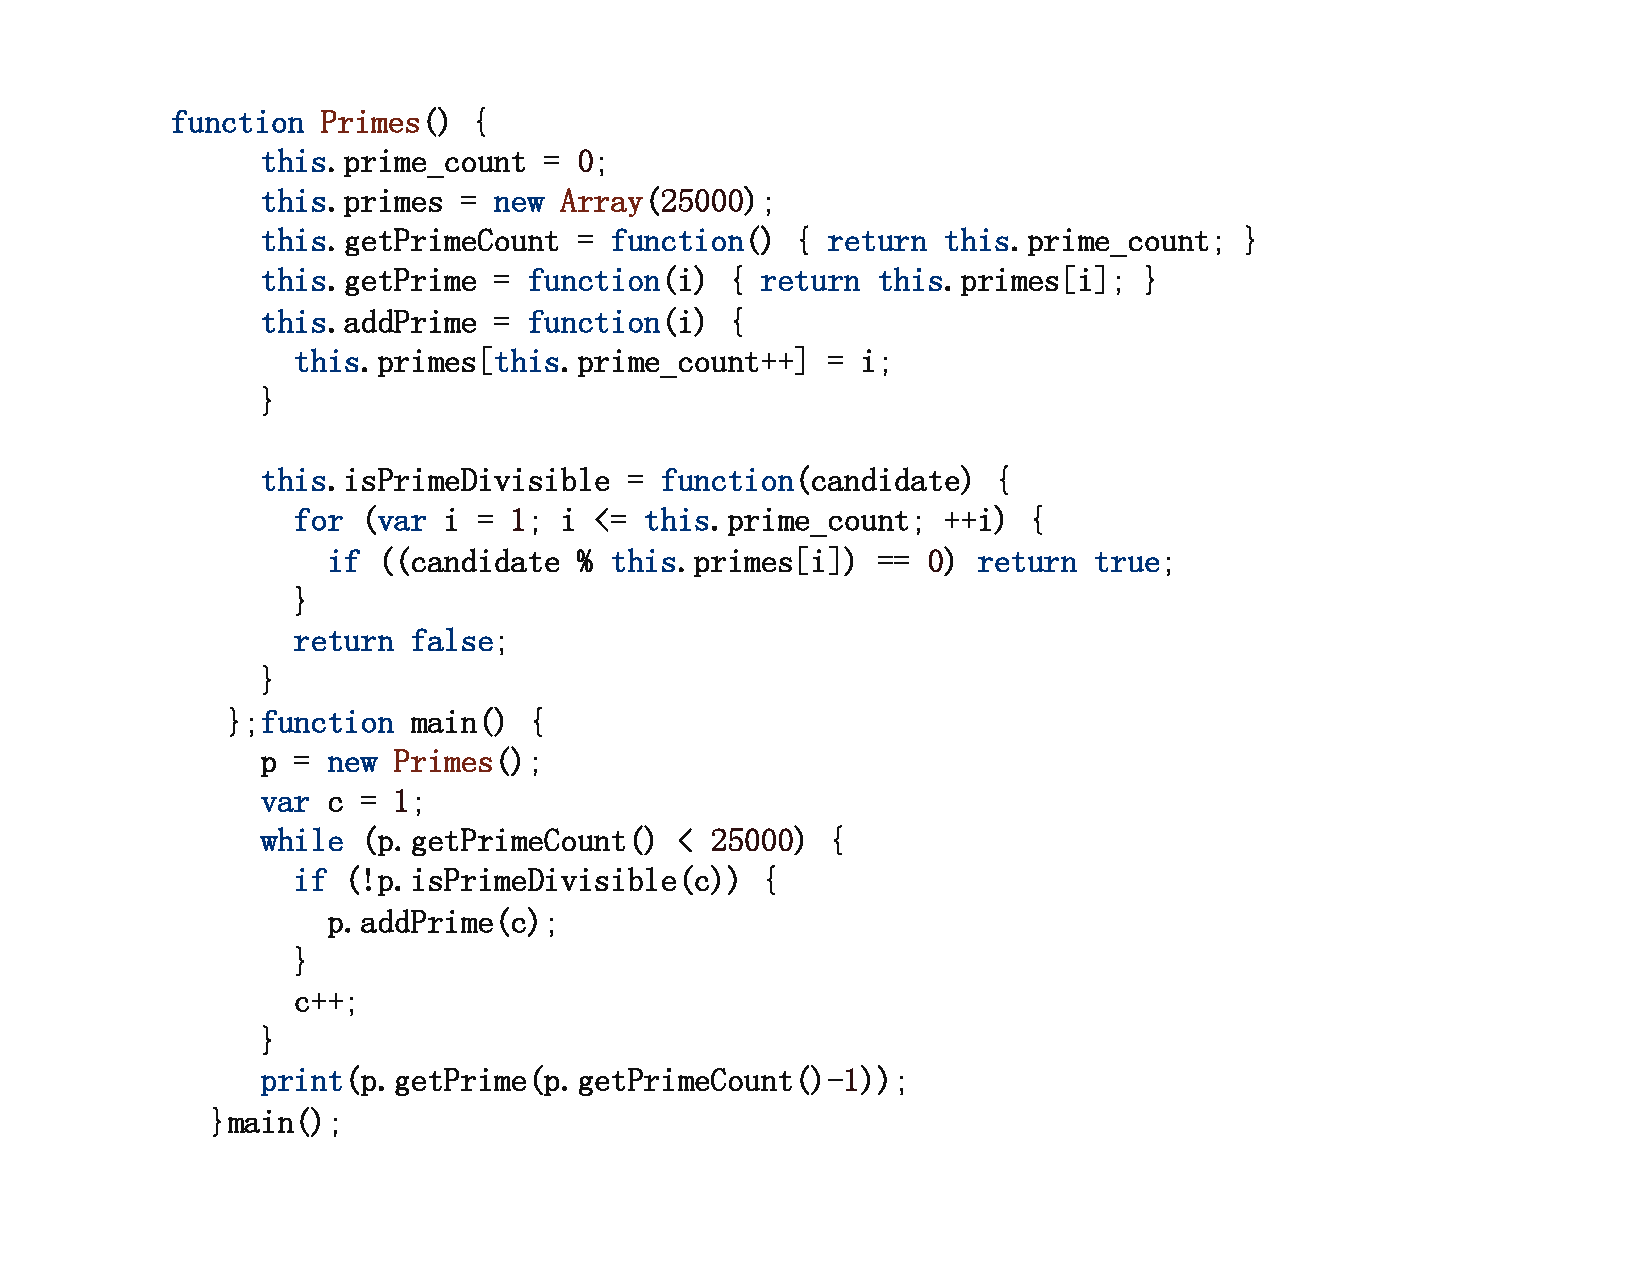
\includegraphics[width=0.44\textwidth]{figs/prime_JavaScript}
        }
    \caption{(a) is the C++ code of calculating the 25000th prime number (b) is the JavaScript code for 25000th prime number.}
 \end{figure}
%
%
%
%\section{Approach}
%
%
%

%
%\section{Results}
%
%\subsection{Experimental Framework}
%
%
%
%\subsection{Data}
%
%
%
%
%
%\begin{table}[h]
%% increase table row spacing, adjust to taste
%\renewcommand{\arraystretch}{1.3}
%\caption{There is no period in a table caption}
%\label{table_example}
%\centering
%% Some packages, such as MDW tools, offer better commands for making tables
%% than the plain LaTeX2e tabular which is used here.
%\begin{tabular}{|c||c|}
%\hline
%One & Two\\
        %\hline
        %Three & Four\\
            %\hline
            %\end{tabular}
            %\end{table}
            %\renewcommand{\arraystretch}{1}
            %
            %\section{Related Work}
            %
            %
            %
            %\section{Conclusion}
            %
            %
            %
            %\section*{Acknowledgment}


            \begin{thebibliography}{1}

            %\bibitem{IEEEhowto:kopka}
            %H.~Kopka and P.~W. Daly, \emph{A Guide to \LaTeX}, 3rd~ed.\hskip 1em plus
            %  0.5em minus 0.4em\relax Harlow, England: Addison-Wesley, 1999.
            \bibitem{Trace}
            Jungwoo Ha and Mohammad R. Haghighat and Shengnan Cong, A concurrent trace-based just-in-time compiler for javascript, Tech Report, 2009
            \bibitem{Popularity}
            John Garofalakis and Panagiotis Kappos and Dimitris Mourloukos, Web site optimization using page popularity, Internet Computing, 1999
            \bibitem{node}
            "Why Everyone Is Talking About Node." Jolie O'Dell. Mashable, Inc., Web. 10 Mar. 2011.

            \end{thebibliography}




            % that's all folks
            \end{document}


